\section{Framework Components}
\label{sec:framework}
Current collaborative robot solutions guarantee safety, but they use
obstacle detection to stop moving. Our dynamic obstacle avoidance
solution is that of using obstacle detection to respond by moving around the
obstacles while continuing to accomplish the desired tasks. Additionally, the integrated dynamic motion planning approach creates motion
plans that fulfil various task specific constraints for typical industrial
applications. For example the work cell 3D model is used to create a consistent
model of the work environment, so that collision free trajectories are flexibly 
generated for different operations. The automatic consideration of these
constraints  drastically simplifies and speeds-up the deployment of the robot.

An artist's illustration of the proposed dynamic obstacle avoidance solution is shown
in Fig. \ref{fig:overview}. The robot motion control component generates
appropriate motion commands for the robot controller to follow the trajectories required for a given task. The proximity-sensing skin that covers the links and joints of the manipulator, produces information regarding potential collisions. This information is used by the robot motion control
module to adapt the robot motions on the fly to fulfil both constraints:
following the current trajectory (with a certain tolerance) and avoid
collisions. If the collision is unavoidable with local deformations of the
current trajectory, the robot motion control module requests a (global) re-planning,
which is performed on the fly by the reactive path-planner. The motion control
then takes the end effector to the final goal pose using the alternative
trajectory. 

\begin{figure}[t]
\centering
\resizebox{0.8\columnwidth}{!}{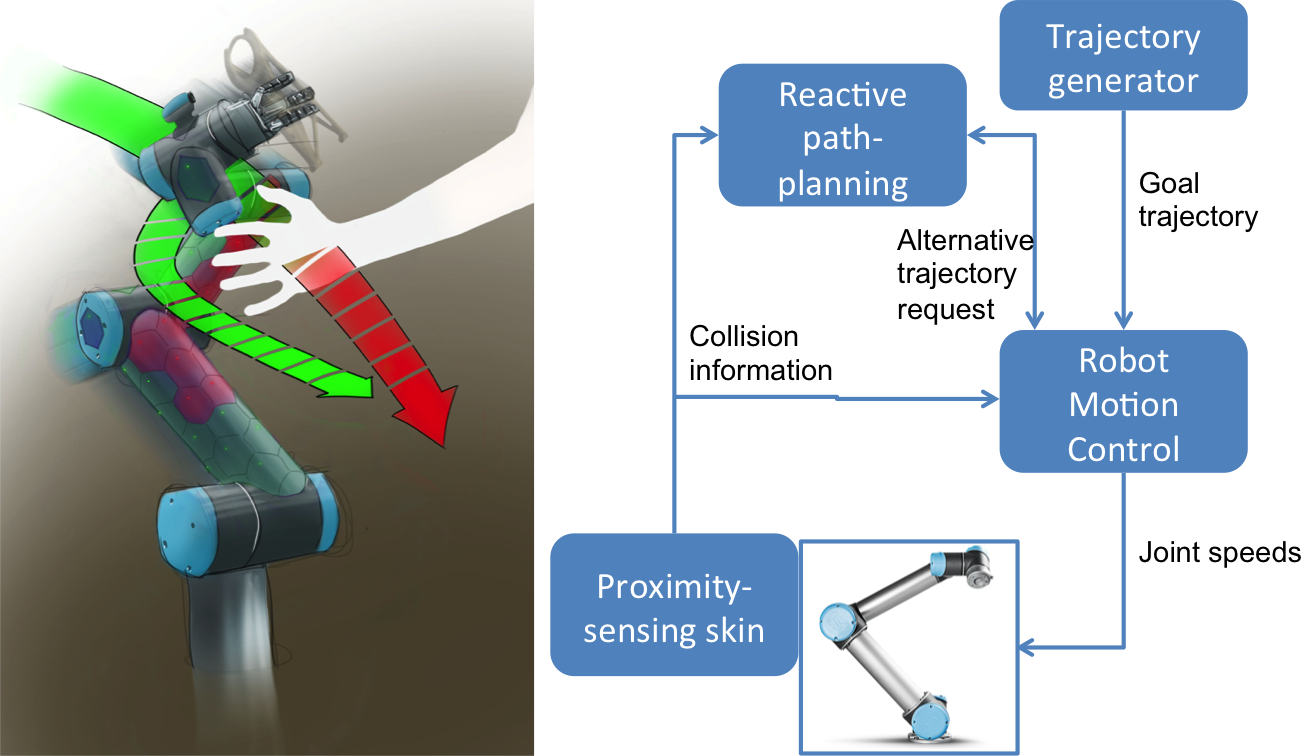
\includegraphics{doa/images/overview.png}}
\caption[]{An artist's schematization of the FiaD Dynamic obstacle avoidance
concept is illustrated on the left side. On the right, an overview of the main
components of the solution.}
\label{fig:overview}

\end{figure}

\begin{figure}[h]
\centering
\resizebox{0.8\columnwidth}{!}{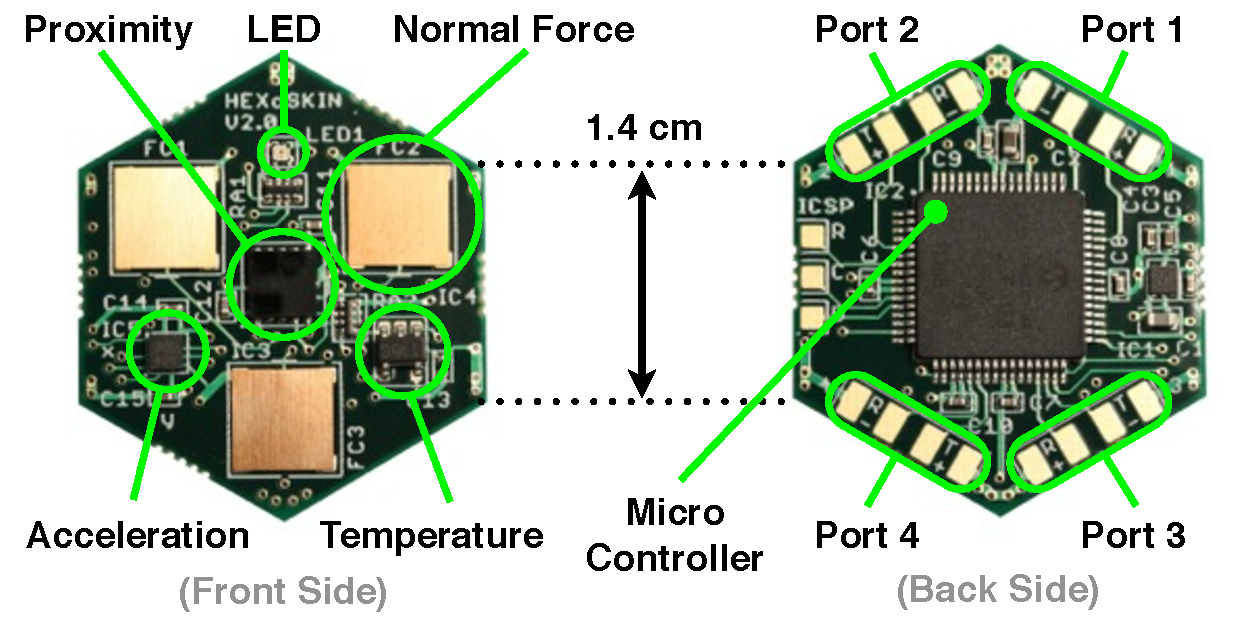
\includegraphics{doa/images/sensor_unit.pdf}}
\caption[]{Robot skin developed at Institute for Cognitive Systems (ICS), TUM.}
\label{fig:RobotSkin}
\vspace{-10pt}
\end{figure}	

\subsection{Artificial Robot Skin}
The robot skin system is modularized and transduces multi-modal tactile stimuli \cite{MittendorferYC15}. The robot skin consists of hexagonally shaped PCB modules called skin cells (see Fig. \ref{fig:RobotSkin}). A group of directly connected skin cells is termed skin patch. All skin cells are identical and contain the same set of sensors. The sensors sample 9 tactile stimuli of 4 different modalities, namely vibration (3D acceleration sensor), 3 normal forces (capacitive force sensor), 2 temperatures and 1 distance (optical proximity sensor). These sensors are either off-the-shelf standard ICs or in the case of the force sensors a in-house development. A micro-controller in the back of each skin cell collects data from its sensors, filters it and creates and sends data packets, which contain the most recent values of all sensors. All the skin cells are connected to each other via stretchable flex PCBs which allows the skin to cover curved surfaces and increases its robustness. The network of skin cells is a meshed bidirectional communication network which is routed by the micro-controllers of the skin cells. A self-organized algorithm initializes all the skin cells in a skin network and constructs a bidirectional communication path between each skin cell and the network root, the tactile section unit (TSU). The TSU converts skin network packets to standard UDP Ethernet packets and vice versa. This allows for fast low latency connections between robot skin and PC (see Fig. \ref{fig:SkinCellNetworkArchitecture}).
\begin{figure}[t]
\centering
\resizebox{0.8\columnwidth}{!}{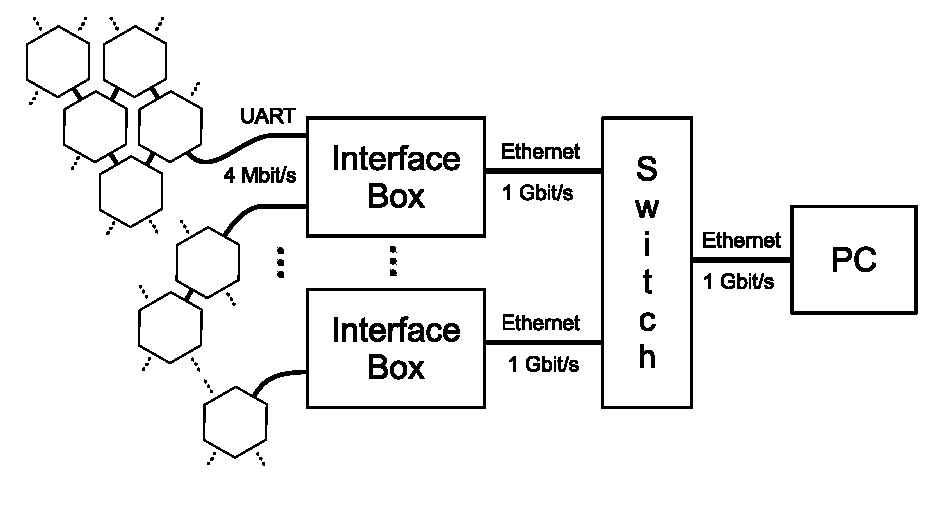
\includegraphics{doa/images/SkinCellNetwork.pdf}}\\[-15pt]
\caption[]{The skin cell network architecture and interface to the PC.}
\label{fig:SkinCellNetworkArchitecture}
\vspace{-10pt}
\end{figure}
The robot skin system also supports the auto-calibration of spatial relationships between skin cells of a skin patch covering a 3D 
surface \cite{Mittendorfer-IROS12tendorfer} such that the kinematic chain of every skin cell to the base frame can easily be determined.  

The proximity sensors used in the skin cells are infrared based sensors. The sensor emits infrared light and captures its reflections on obstacles 
in the range from 0 to 15 cm. The strength of the reflections allows the sensor to estimate the distance between the sensor and detected objects.  

\paragraph{Evaluation of Artificial Robot Skin}
\begin{figure}[h]
\centering
\resizebox{1.0\columnwidth}{!}{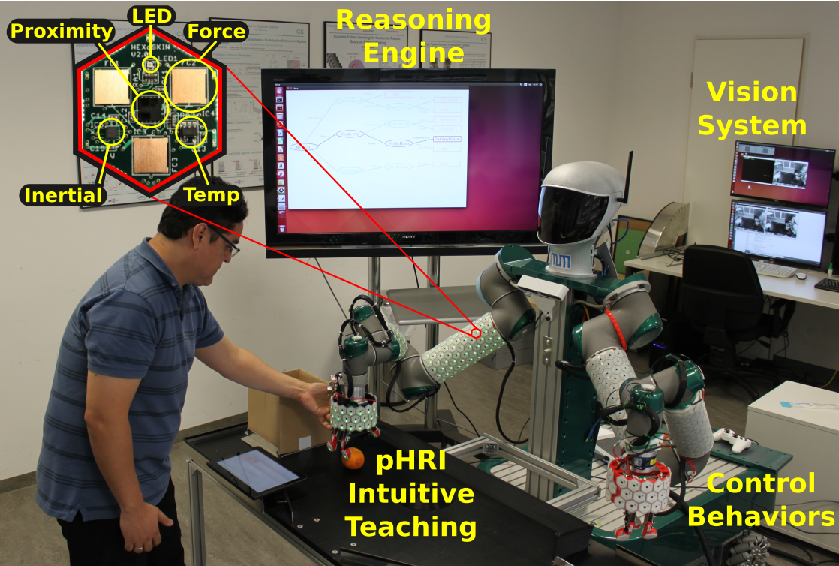
\includegraphics{doa/images/Demo.pdf}}\\[-10pt]
\caption[]{Robot TOMM. Its arms and grippers are covered with artificial robot skin. the figure depicts the robot in an industrial scenario.}
\label{fig:TommSorting}
\end{figure}

\begin{figure}[h]
\centering
\resizebox{1.0\columnwidth}{!}{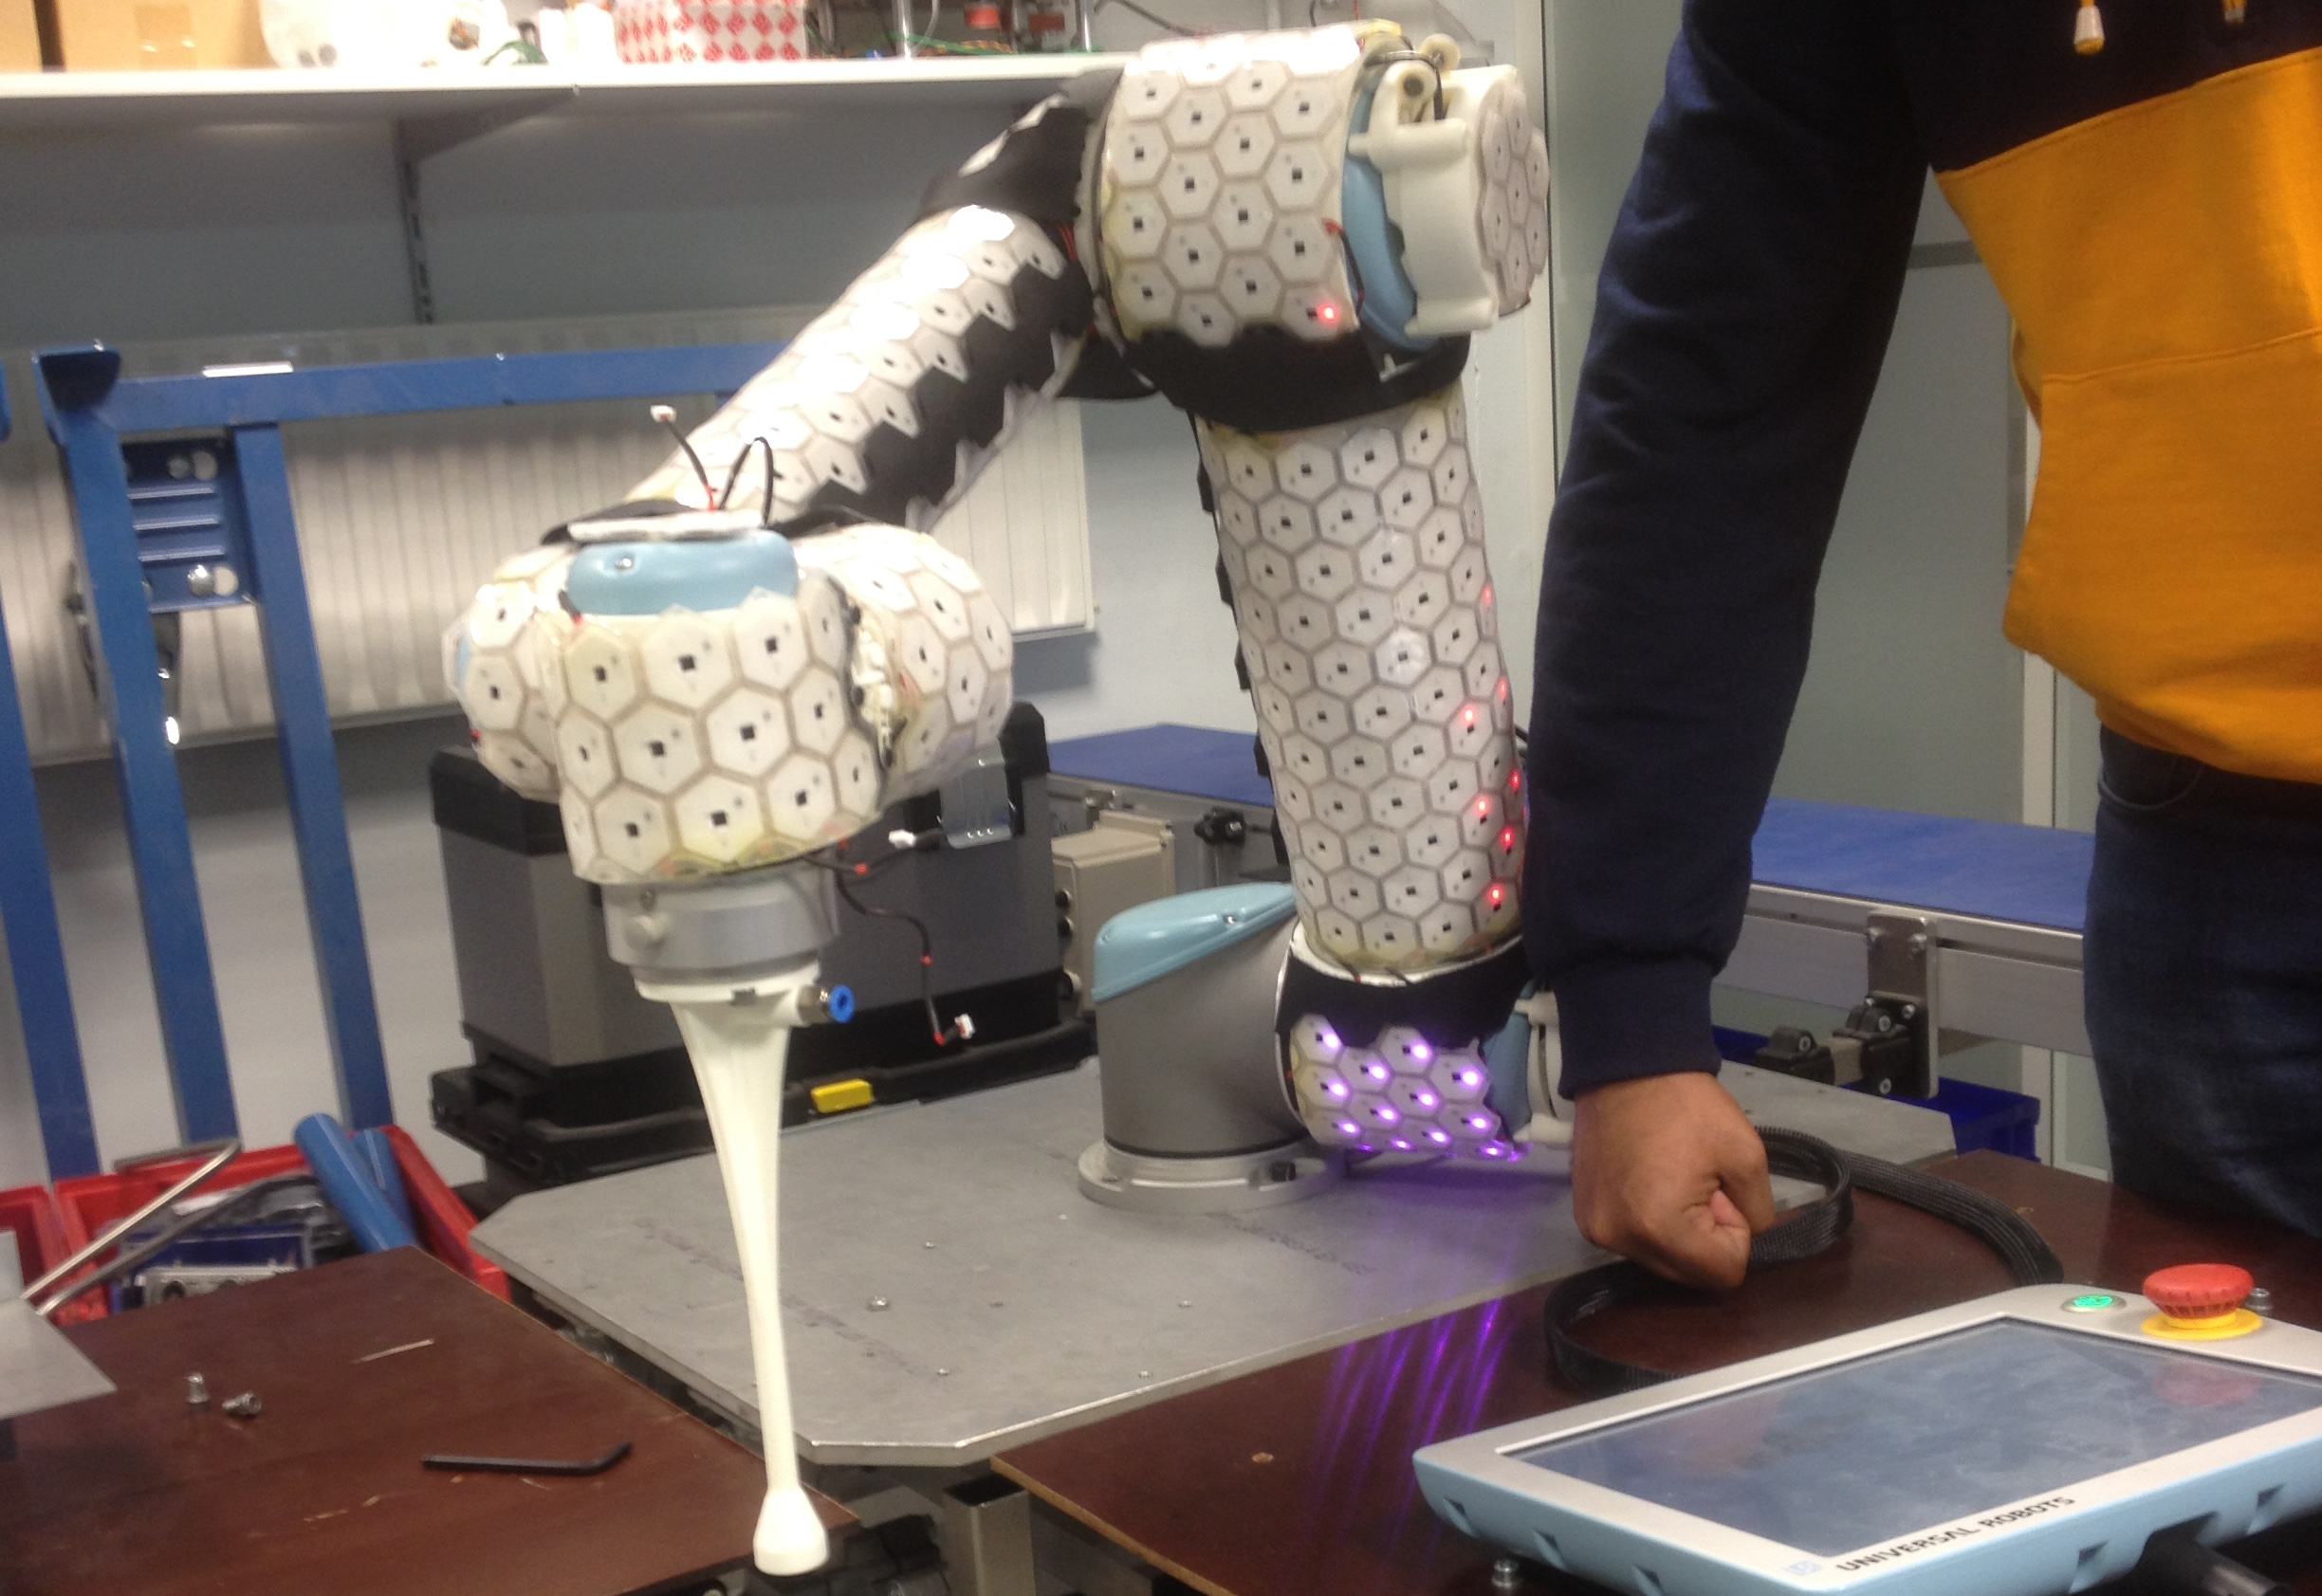
\includegraphics{doa/images/TUD_Setup.JPG}}\\[-10pt]
\caption[]{UR5 setup showing Artificial Skin Cells being activated (with red LEDs) by obstacles ($<= 6\,cm$).}
\label{fig:TUDSetup}
\end{figure}

The \textit{Artificial Robot Skin} (ARS) has been successfully deployed on the robot TOMM \cite{Dean-ICRA17} (see Fig. \ref{fig:TommSorting}). The integration of the multi-modal artificial skin signals in the control loop of the arms is demonstrated in \cite{Dean-Humanoids16} where the self-calibrating artificial skin framework is used to control the dynamic behavior of the industrial robot, e.g. producing compliance in a non-compliant robot. The advantage of these compliant behaviors is to generate safer robots, especially for physical Human-Robot Interaction. The fusion of the multi-modal signals of the artificial skin with different sensors (e.g. cameras and joint encoders) in a semantic level is demonstrated in \cite{Ramirez-Amaro-Humanoids16}. These semantic representations are used to extract general task structures which together with the obtained knowledge can improve and accelerate teaching of new tasks \cite{Dynaov-Humanoids16}. Finally, the integration of these technologies has been evaluated in an industrial scenario, where a human can kinesthetically teach the robot TOMM to sort oranges \cite{Dean-IECON16} (see Fig. \ref{fig:TommSorting}).

ARS has also been deployed successfully on another practical setup with a statically mounted Universal Robots UR5 robot (see Fig. \ref{fig:TUDSetup}). In this setup, the ARS is being used to provide proximity information related to obstacles in the immediate surroundings of the robot.


\section{Reactive Controller}
The motion control is achieved using the Stack of Tasks (SoT) controller
framework \cite{Mansard2009} which employs a hierarchical jacobian control strategy eliminating the analytical inverse kinematics computation thus making it a generic controller for all robot platforms. The controller's hierarchical nature allows the robot to handle multiple kinematic tasks simultaneously exploiting the kinematic redundancy of the robot. The controller's real time capability comes from the high computational speed of the state of the art Hierarchical Quadratic Programming (HQP) solver backing it. 


A \emph{task} basically is a control law that achieves a specific objective which can be a free space task or just an inequality constraint that narrows down the workspace of the robot. The task function formalism is very well discussed in \cite{C.Samson1991}. In the context of our work, tasks generally include robot joint posture task, collision avoidance task, joint limits task and so on. The SoT framework handles the task priorities hierarchically in the real time to ensure there are no conflicts among tasks which is used to achieve dynamic obstacle avoidance without compromising on the main goal.

For example, let us consider a pick and place application in a collaborative
environment. The primary goal for this application is to enable a robot to move
to a (set of) desired pick and place locations repetitively. The pick and place
locations can be defined as posture tasks in SoT. However, a higher priority
task considering the collaborative nature of the environment is to avoid
collisions with obstacles that could be humans, for instance. Typically such a
task is modelled as an ``Inequality'' task and an eventual feasible solution (if
one exists) is computed by the solver by exploiting the kinematic redundancy of the robot. In the jargon of motion planning and control, this behavior is similar to a \emph{local planner}.
However, it is likely that a feasible solution is not found due to the solver
converging to a local minima\footnote{This is caused by the use of task
Jacobians. For further details, please see \cite{Mansard2009}.} In such a
scenario, SoT can also be used to leverage the services of a global planner (see
Section \ref{subsec:react_path}) from the current robot state to the goal so
that an entirely new path is obtained which is free from collisions and
consequently allowing all the specified tasks to be achieved in the order of
their priorities. In Section \ref{sec:prelim_results}, we present the
experimental results of using the SoT controller on a practical setup and in
simulation. The SoT controller has also been configured to work with the ROS-control interface. In all these setups, the proximity information from
the artificial robot skin is used as an input to the collision avoidance task. In
the following part, we briefly present the global path planner software framework
that is used when the SoT controller hits a local minima.
\begin{figure}[t]
\centering
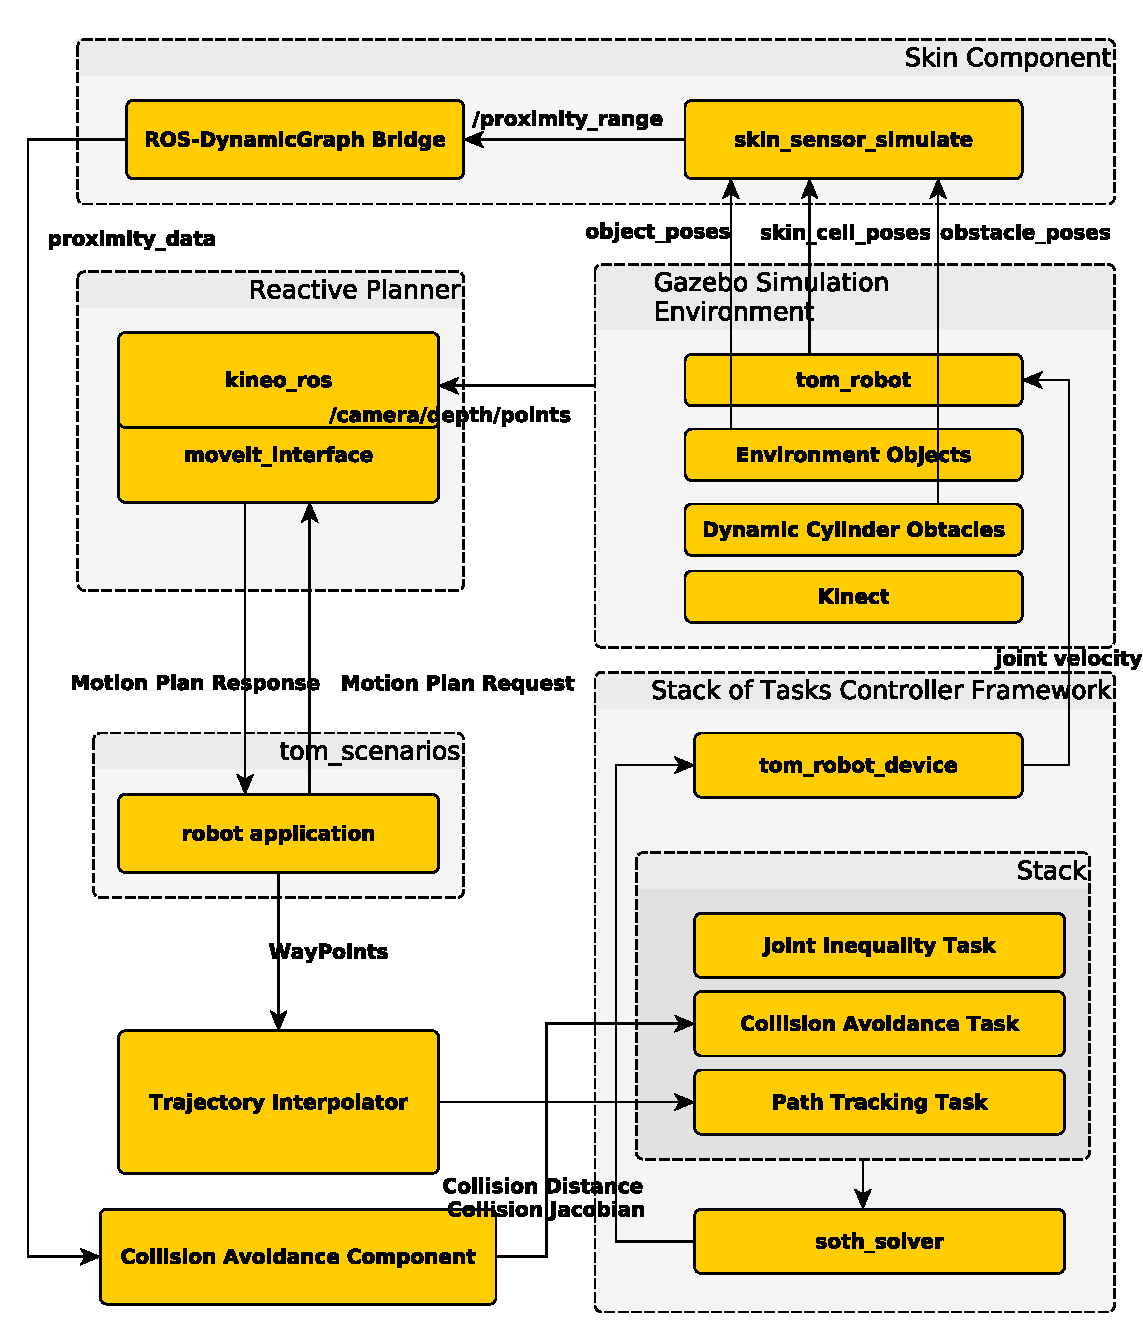
\includegraphics[scale=0.47]{doa/images/architecture_reactive_collision_1.pdf}
% \resizebox{2\columnwidth}{!}{\includegraphics{arch_tom_3}}\\
\caption[]{Dynamic collision avoidance software architecture.}
\label{fig:dca}
\end{figure}

\section{Reactive Motion Planning}
\label{subsec:react_path}
\hypersetup{colorlinks, linkcolor=blue}
The reactive path planning software framework is based on the industry grade KineoWorks\texttrademark\footnote{See
\href{http://www.plm.automation.siemens.com/en\_us/products/open/kineo/kineoworks/index.shtml}{Kineoworks}.} path planning library from Siemens in order to provide fast and reliable robot paths. This framework has also been seamlessly integrated into the ROS-ecosystem via a ROS package called \texttt{kws\_ros\_interface} which provides the planner implementations of KineoWorks as shared objects that are readily usable in ROS-based software via the \texttt{kws\_ros\_planner} ROS node.

Robot kinematic models are provided to KineoWorks in the Unified Robot Description Format (URDF) which is a ROS standard. Furthermore, KineoWorks also accepts the standard ROS representation of a \texttt{PointCloud}\footnote{See http://wiki.ros.org/pcl} for creating collision models of dynamic obstacles in the environment. The point clouds are generated in two ways. In one scenario the point clouds are generated by a standard Kinect 3D camera that is observing the immediate environment of the robot. In the other scenario, the point clouds are generated from the proximity data obtained from the Artificial Skin. Finally, the collision detection for dynamic obstacle avoidance is performed using the Kineo\texttrademark Collision Detector (KCD)\footnote{See \href{http://www.plm.automation.siemens.com/en\_us/products/open/kineo/collision-detector/index.shtml}{KCD}.}. KCD performs 3D collision detection and minimal distance analysis between triangular mesh surfaces in assembly environments. KCD has been designed specifically to minimize memory usage and take advantage of parallel processing. The complete software architecture used for the Dynamic Collision Avoidance capability is shown in Fig. \ref{fig:dca}.

